\section{Evaluation}\label{sec:experiments}
\subsection{Setup}
\subsubsection{Environment}
The experiments were performed on a single machine with two Intel Xeon Processor E5--2699 v4 CPUs, 64 GB of RAM,
and an 800GB SSD\@.
The machine has 22 cores and 44 threads.
In memory data caches for file system were dropped before each experiment to force disk loads.

Table~\ref{tab:disk} shows the performance baseline of the SSD that we use.
The baseline is tested by fio (2.2.10).
Each testcase reads/writes 1GB data within 10min.
\begin{table}
  \caption{Disk Performance Baseline}\label{tab:disk}
  \begin{tabular}{rrr}
    \toprule
    mode-blocksize-iodepth-numjobs & Read (MB/s) & Write (MB/s) \\
    \midrule
    Seq-1M-8--1    & 474.99 & 467.89 \\
    Seq-128K-32--1 & 480.58 & 458.24 \\
    Rnd-4K-32--16  &  17.11 &  12.83 \\
    Rnd-4K-1--1    &  33.56 &  97.37 \\
    \bottomrule
  \end{tabular}
\end{table}
\subsubsection{Datasets and Queries}
Our datasets and the queries have 2 vertex labels and 2 edge labels.
We use real-world data graphs~\cite{snapnets} listed in Table~\ref{tab:datasets} with different sizes. The vertices and edges in the datasets are labeled randomly as in~\cite{DBLP:journals/pvldb/MhedhbiS19}.
The queries (Figure~\ref{img:queries}) are selected from existing work~\cite{DBLP:conf/cloud/SerafiniMS17,DBLP:journals/pvldb/MhedhbiS19}.
The labels of vertices and edges are tagged randomly,
and they are represented by the colors and patterns of lines in Figure~\ref{img:queries}.
The queries we choose represent different topologies: trees, chains, and cyclic graphs.
$q_9$ --- $q_{12}$ are queries with multi-edges.
\begin{table}
  \caption{Datasets}\label{tab:datasets}
  \begin{tabular}{lrr}
    \toprule
    Name & $|V|$ & $|E|$ \\
    \midrule
    soc-Epinions (EP) & 76K & 509K \\
    web-Google (GO) & 876K & 5.1M \\
    web-BerkStan (BS) & 685K & 7.6M \\
    soc-LiveJournal (LJ) & 4.8M & 69M \\
    com-Orkut (OK) & 3.1M & 117.2M \\
    \bottomrule
  \end{tabular}
\end{table}

\begin{figure}[ht]
  \centering
  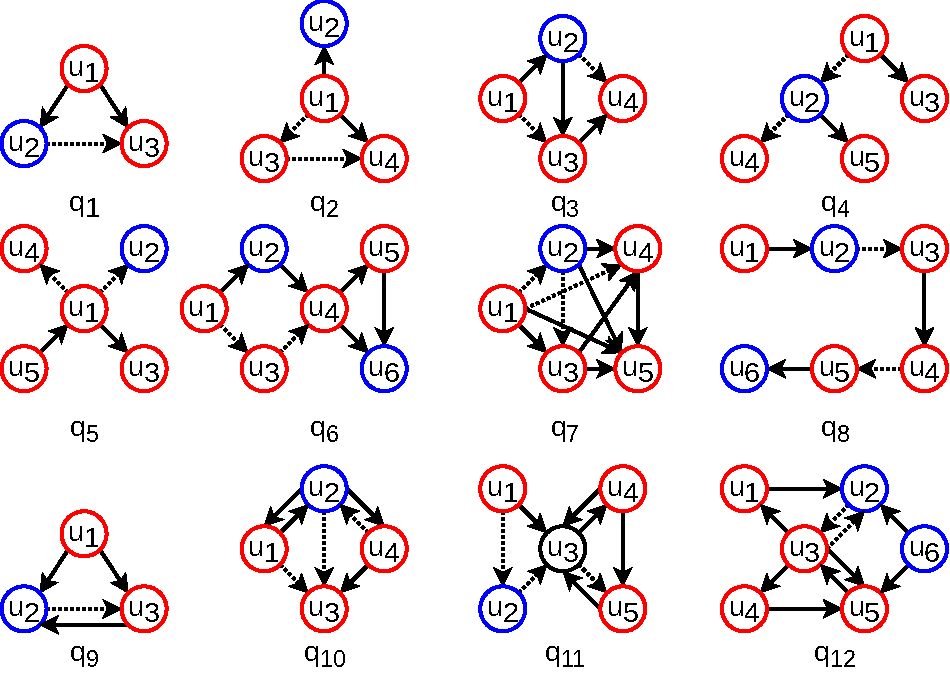
\includegraphics[width=0.5\textwidth]{img/queries.pdf}
  \caption{The queries.}\label{img:queries}
\end{figure}

\subsection{Preprocessing Cost}
We first study the preprocessing cost of SeqStar's vertex-centric storage engine.
The preprocessing incurs an external sort on the original graph data to generate the formatted data graph shown in Figure~\ref{img:data_graph}.
The cost is $\mathcal{O}(n \log n)$ where $n$ is the size of the unsorted graph data.
We use 32-bit integers to store the vertex IDs, and 16-bit integers to store the vertex/edge labels.
As is shown in Figure~\ref{img:exp_preprocessing}, the preprocessing time grows linearly with respect to the size of graph data.
In fact, the preprocessing time of the vertex-centric storage is significantly smaller than the execution time of complex queries (\S\ref{sec:experiments_compare}).

\begin{figure}[ht]
  \centering
  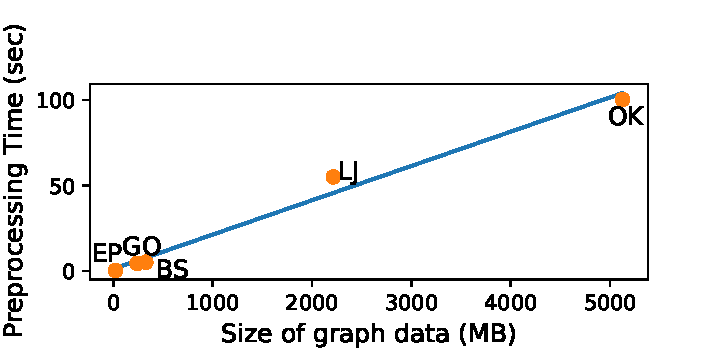
\includegraphics[width=0.4\textwidth]{img/exp_preprocessing.pdf}
  \caption{Preprocessing time of SeqStar.}\label{img:exp_preprocessing}
\end{figure}
\subsection{Comparative Performance}\label{sec:experiments_compare}
We evaluate the performance of SeqStar, Graphflow and Neo4j (Version 4.2.3).
Graphflow is the state-of-the-art in-memory subgraph querying system,
and it is the fastest baseline we are aware of.
Graphflow is a JVM based system, and we set the maximum size of the JVM heap to 60GB to full use of the main memory.
However Graphflow does not support queries with multi-edges, i.e., $q_9$ --- $q_{12}$,
and it will report fake results for these queries\footnote{Graphflow will report matchings even the data does not contain multi-edges.}.
Therefore we use $q_1$ --- $q_8$ to compare to Graphflow.
Neo4j is a widely used industrial graph database, which fully supports the property graph model.
However, Neo4j runs much slower than Graphflow and SeqStar for graph matching.
Therefore we only test $q_9$ --- $q_{12}$  on Neo4j that Graphflow doesn't support.

\begin{figure*}[ht]
  \centering
  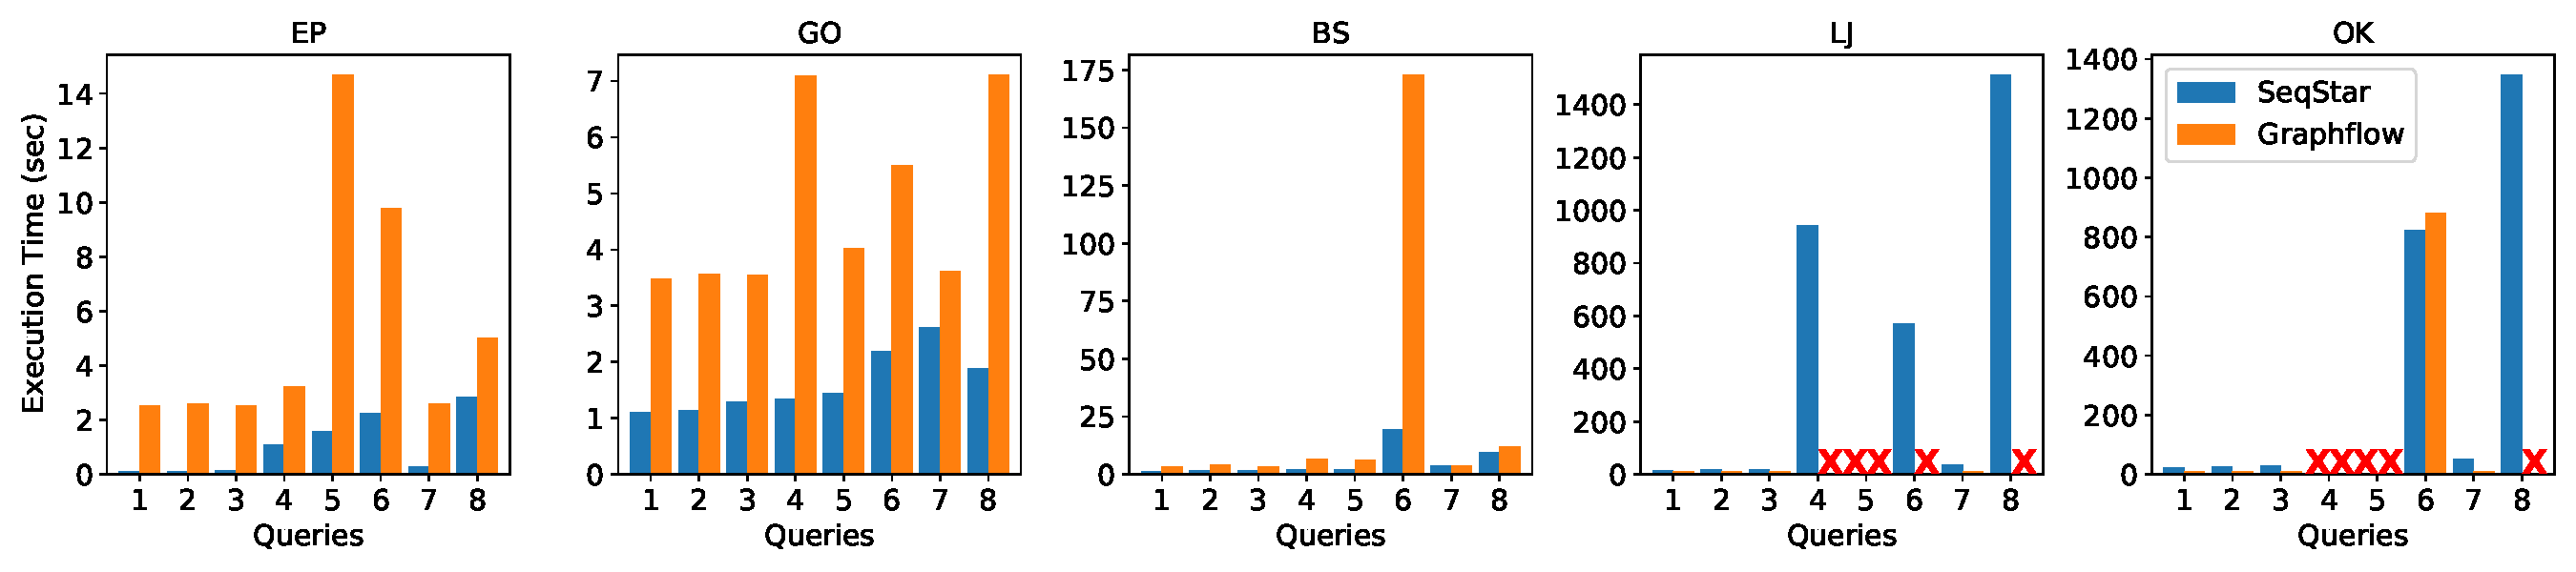
\includegraphics[width=\textwidth]{img/exp_compare.pdf}
  \caption{Execution time of SeqStar and Graphflow.}\label{img:exp_compare}
\end{figure*}

Figure~\ref{img:exp_compare} compares SeqStar against Graphflow.
For datasets EP, GO and BS, SeqStar outperforms the existing work by $1.4\times$ to $26\times$.
Graphflow uses edges as the basic matching unit and applies worst case optimal join on the edges.
In contrast, our SeqStar use stars to filter the graph data.
As stars contain more filtering constraints than edges, SeqStar results in smaller intermediate results.
Moreover, SeqStar compresses the intermediate results and performs parallel pipeline join on the compressed data.
Therefore, the memory usage of SeqStar is much smaller than Graphflow,
and the time spent on processing the intermediate data is reduced.
%% We notice that the CPU utilization of Graphflow drops quickly as some cores finish their work early,
%% leading to the long tail problem.
%% In contrast, SeqStar overcomes the long tail problem by work stealing and our SeqStar is the clear winner.

For datasets LJ and OK, the datasets are so large that the disk scanning overhead of SeqStar predominates as the datasets become larger.
Therefore Graphflow outperforms SeqStar on $q_1$, $q_2$, $q_3$ and $q_7$.
However, for complex query such as $q_6$, SeqStar still outperforms Graphflow in dataset OK\@.
Moreover, Graphflow fails to process $q_4$, $q_6$ (except dataset OK) and $q_8$ due to the out of memory problem.
Whereas our SeqStar still works on these queries.
Both SeqStar and Graphflow fail to finish enumerating $q_5$ in 35 minutes as the result size is quite large:
there are $3.2 \times 10^{13}$ rows of final results for LJ and $3.8 \times 10^{14}$ rows for OK\@.
However, our SeqStar is able to analyze the compressed data and report useful information,
e.g., the result size for LJ and OK on $q_5$ can be reported in less than 20 seconds
(SeqStar scans the SuperRows and uses the formula $|s_1 \times s_2 \times \cdots| = |s_1| \times |s_2| \times \cdots$ to calculate the size of Cartesian products without performing the actual product operation).

Figure~\ref{img:exp_compare_neo4j} shows the execution time of SeqStar and Neo4j on query $q_9$ to $q_{12}$.
The dataset OK does not contain multi-edges and we omit it in this experiment.
Neo4j fails to get the final answer of $q_{11}$, $q_{12}$ on BS, and $q_{10}$ --- $q_{12}$ on LJ in 35min.
Our SeqStar outperforms Neo4j by up to 3 orders of magnitude.
\begin{figure}[ht]
  \centering
  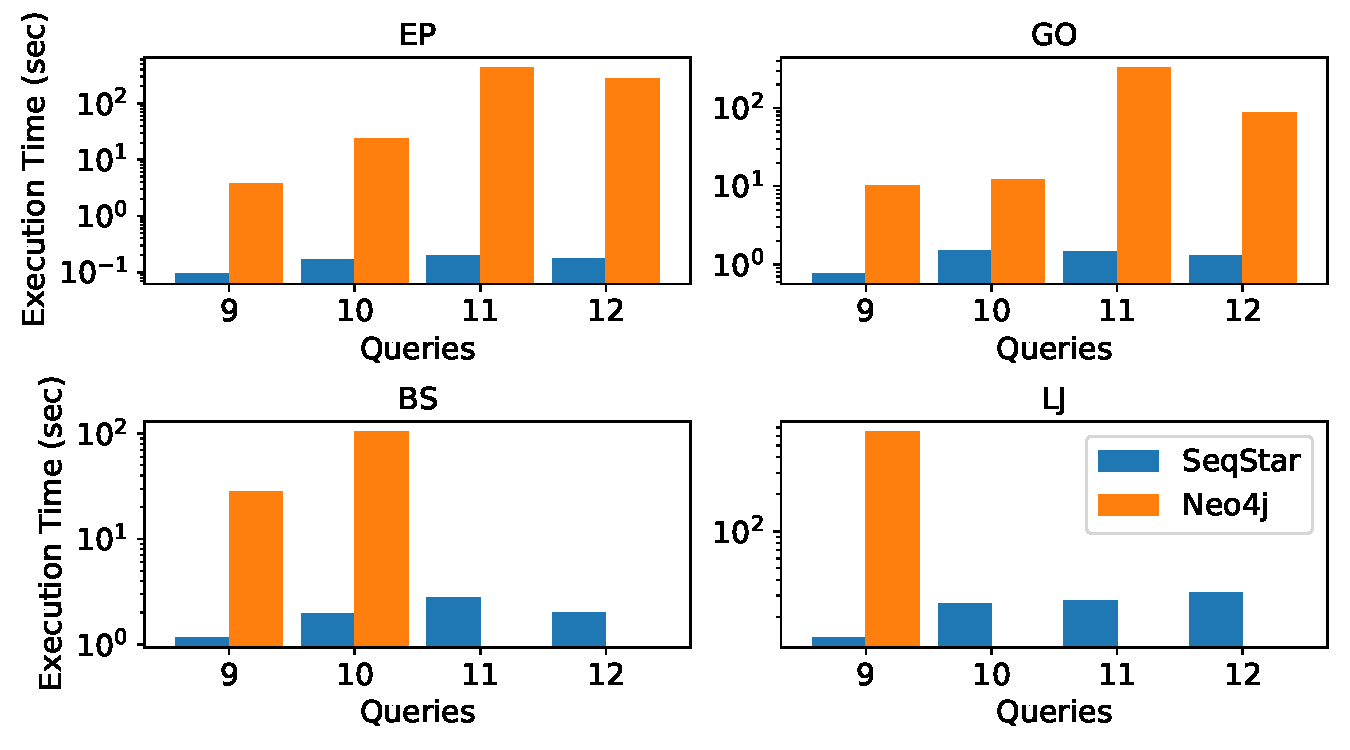
\includegraphics[width=0.45\textwidth]{img/exp_compare_neo4j.pdf}
  \caption{Execution time of SeqStar and Neo4j.}\label{img:exp_compare_neo4j}
\end{figure}
\subsection{Compression Ratio}\label{sec:experiments_compress}
Table~\ref{tab:compressed} shows the size of compressed intermediate results (SuperRows).
The size of the SuperRows (include metadata) is much smaller (less than $22\%$) compared to the size of the original graph data (Figure~\ref{img:exp_preprocessing}).
SeqStar will only generate intermediate results from star matching,
and they can be cached in memory to boost queries.

\begin{table}
  \caption{Size of compressed intermediate results. (MB)}\label{tab:compressed}
  \begin{tabular}{lrrrrr}
    \toprule
    $q$ &  EP &  GO &  BS &  LJ &  OK \\
    \midrule
    1  &   1 &  15 &  19 & 174 & 267 \\
    2  &   2 &  16 &  21 & 208 & 317 \\
    3  &   2 &  15 &  19 & 238 & 366 \\
    4  &   1 &  16 &  20 & 206 & 314 \\
    5  &   1 &   9 &  11 & 153 & 240 \\
    6  &   3 &  29 &  37 & 411 & 619 \\
    7  &   4 &  33 &  43 & 477 & 749 \\
    8  &   3 &  25 &  31 & 343 & 505 \\
    9  &   1 &   6 &   8 & 119 & 0 \\
    10 &   2 &  13 &  16 & 244 & 0 \\
    11 &   2 &  14 &  18 & 249 & 0 \\
    12 &   2 &  11 &  14 & 251 & 0 \\
    \bottomrule
  \end{tabular}
\end{table}

Table~\ref{tab:compression_ratio} shows the compression ratio of SeqStar's SuperRow.
The compression ratio is calculated by as \emph{(uncompressed data size) / (compressed data size)}.
In the table, $93\%$ of the data have a compression ratio larger than $10$;
$73\%$ larger than $100$; and $59\%$ larger than $1000$.

We also studied the impact of metadata in SuperRows (described in \S\ref{sec:match_compress}, also in Figure~\ref{img:compress}),
and find that the metadata takes no more than $35\%$ of the space for intermediate results.
Over $68\%$ of the cases, the metadata use less than $25\%$ of the space.

\begin{table}
  \caption{The compression ratio of SuperRows.}\label{tab:compression_ratio}
  \begin{tabular}{lrrrrr}
    \toprule
    $q$ &     EP &       GO &          BS &       LJ &        OK \\
    \midrule
    1  &     26 &       35 &         699 &       37 &        90 \\
    2  &   2225 &       15 &         114 &     9227 &    174687 \\
    3  &   1603 &      207 &        5645 &     3373 &      6823 \\
    4  &    812 &       13 &         114 &     2154 &      6666 \\
    5  & 308241 &      632 &        5144 &  3966263 &  30030074 \\
    6  &  59045 &     1091 &       28381 &   353610 &   1031953 \\
    7  & 550049 & 17468015 & 35906569518 & 33560087 & 415665030 \\
    8  &     24 &        4 &          10 &       25 &        31 \\
    9  &     11 &        2 &           7 &       14 &      ---  \\
    10 &   3397 &    37339 &     8700505 &    13089 &      ---  \\
    11 &  10209 &      331 &       14216 &    38987 &      ---  \\
    12 &  11163 &      244 &       13311 &    89171 &      ---  \\
    \bottomrule
  \end{tabular}
\end{table}

\subsection{Parallelism of Pipeline Join}\label{sec:experiments_join}
This section tests the speedup of using multiple cores. The speedup is calculated by the time using a single core divided by the time using multiple cores for a specific query.
%The purpose of this experiment is to study the CPU parallelism of SeqStar's pipeline join.
We choose two of the most time-consuming queries $q_6$ and $q_8$ for the study.
%We use speedup to measure the parallelization effect, which is the elapsed time of the single thread join over that of the multi-threaded execution.

Figure~\ref{img:exp_scalability} shows the speedup of SeqStar's pipeline join by varying the number of threads from 1 to 32.
SeqStar has a nearly linear speedup due to the independence of loops in our pipeline join (\S\ref{sec:match_join}).
Noticeably, SeqStar achieved almost optimal speedup within 8 threads.
Specifically, the speedup of BS $q_6$ is 7.6 using 8 threads and the speedup of GO $q_6$ is 6.7.
\begin{figure}[ht]
  \centering
  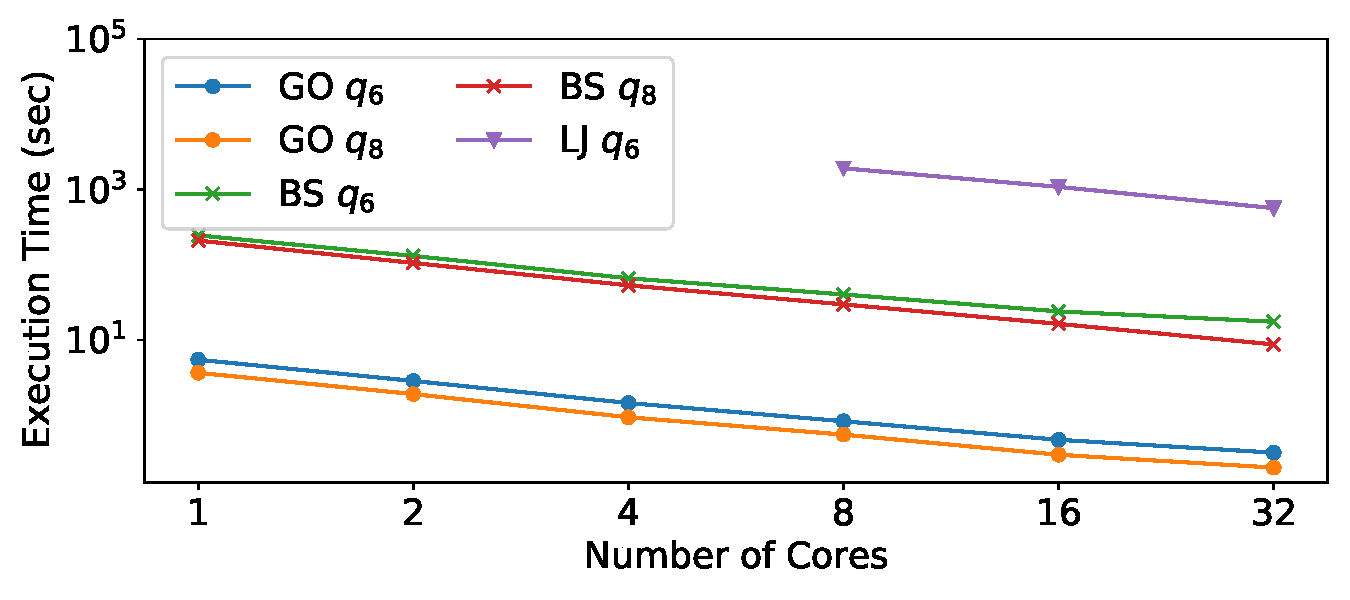
\includegraphics[width=0.5\textwidth]{img/exp_scalability.pdf}
  \caption{Scalability of Pipeline Join.}\label{img:exp_scalability}
\end{figure}

\subsection{Performance of Predicate Pushdown}
In order to understand the benefits of predicate pushdown,
we ran four of the most time-consuming queries $q_4$, $q_5$, $q_6$ and $q_8$ with the following WHERE clause:
\begin{Verbatim}[fontsize=\small]
  WHERE u1 % 5 = 0 AND u2 % u1 = 5
\end{Verbatim}
The analyzer of SeqStar will analyze the WHERE clause and obtain:
(1) a vertex-constraint `$u_1 \bmod 5 = 0$' and (2) an edge-constraint `$u_2 \bmod u_1 = 5$' (\S\ref{sec:match_optimize}).
These constraints can be applied during the star matching process.

Table~\ref{tab:pushdown_lj} and Table~\ref{tab:pushdown_ok} illustrate the effects of predicate pushdown on LJ and OK\@.
$T$ is the execution time with the optimization, i.e., the constraints have to be checked after the graph isomorphism result is obtained.
$T_{OPT}$ is the execution time with predicate pushdown.
$\#R$ is the result size (number of rows) for the queries without the WHERE clause and $\#R_{OPT}$ is the number of rows with WHERE clause applied.

Because of the vertex-constraint `$u_1 \bmod 5 = 0$',
the \textsc{VertexIter} can skip invalid vertices whenever possible.
When scanning the \textsc{NeighborIter}s,
the edge-constraint `$u_2 \bmod u_1 = 5$' is performed to filter out unnecessary matchings.
The star matching time is reduced by $20\%$ --- $62\%$ in these experiments,
and up to $8 \times 10^5 \times$ of unnecessary results are avoided.
As a result, the total execution time obtains a speedup larger than 525$\times$.
\begin{table}
  \caption{Performance of Predicate Pushdown (LJ)}\label{tab:pushdown_lj}
  \begin{tabular}{lrrrrrr}
    \toprule
    $q$ & \parbox{5mm}{$T$ (sec)} & \parbox{5mm}{$T_{OPT}$ (sec)} & $\frac{T}{T_{OPT}}$ & $\#R$ & $\#R_{OPT}$ & $\frac{\#R}{\#R_{OPT}}$ \\
    \midrule
    4 &   944 &        11 &       89 &   $1.0 \times 10^{12}$ &   $6.6 \times 10^7$ &     15376 \\
    5 & >2100 &         4 &     >525 &  $3.2 \times 10^{13}$  &   $6.7 \times 10^8$ &     47520 \\
    6 &   571 &        24 &       24 &   $6.2 \times 10^{11}$ &   $1.6 \times 10^8$ &      3774 \\
    8 &  1513 &        24 &       63 &   $1.7 \times 10^{13}$ &    $2.0 \times 10^9$ &      8512 \\
    \bottomrule
  \end{tabular}
\end{table}

\begin{table}
  \caption{Performance of Predicate Pushdown (OK)}\label{tab:pushdown_ok}
  \begin{tabular}{lrrrrrr}
    \toprule
    $q$ & \parbox{5mm}{$T$ (sec)} & \parbox{5mm}{$T_{OPT}$ (sec)} & $\frac{T}{T_{OPT}}$ & $\#R$ & $\#R_{OPT}$ & $\frac{\#R}{\#R_{OPT}}$ \\
    \midrule
    4 & >2100 &        65 &      >32 &  $5.6 \times 10^{13}$ &   $1.7 \times 10^{10}$ &      3110 \\
    5 & >2100 &         7 &     >300 &  $3.8 \times 10^{14}$ &     $4.6 \times 10^8$ &     813540 \\
    6 &  1399 &        38 &       37 &  $4.4 \times 10^{10}$ &     $8.3 \times 10^5$ &      53035 \\
    8 &  1347 &        36 &       38 &  $1.4 \times 10^{13}$ &     $6.1 \times 10^8$ &      22609 \\
    \bottomrule
  \end{tabular}
\end{table}

